\documentclass{standalone}
\usepackage{tikz}
\usetikzlibrary{patterns, positioning}

\begin{document}
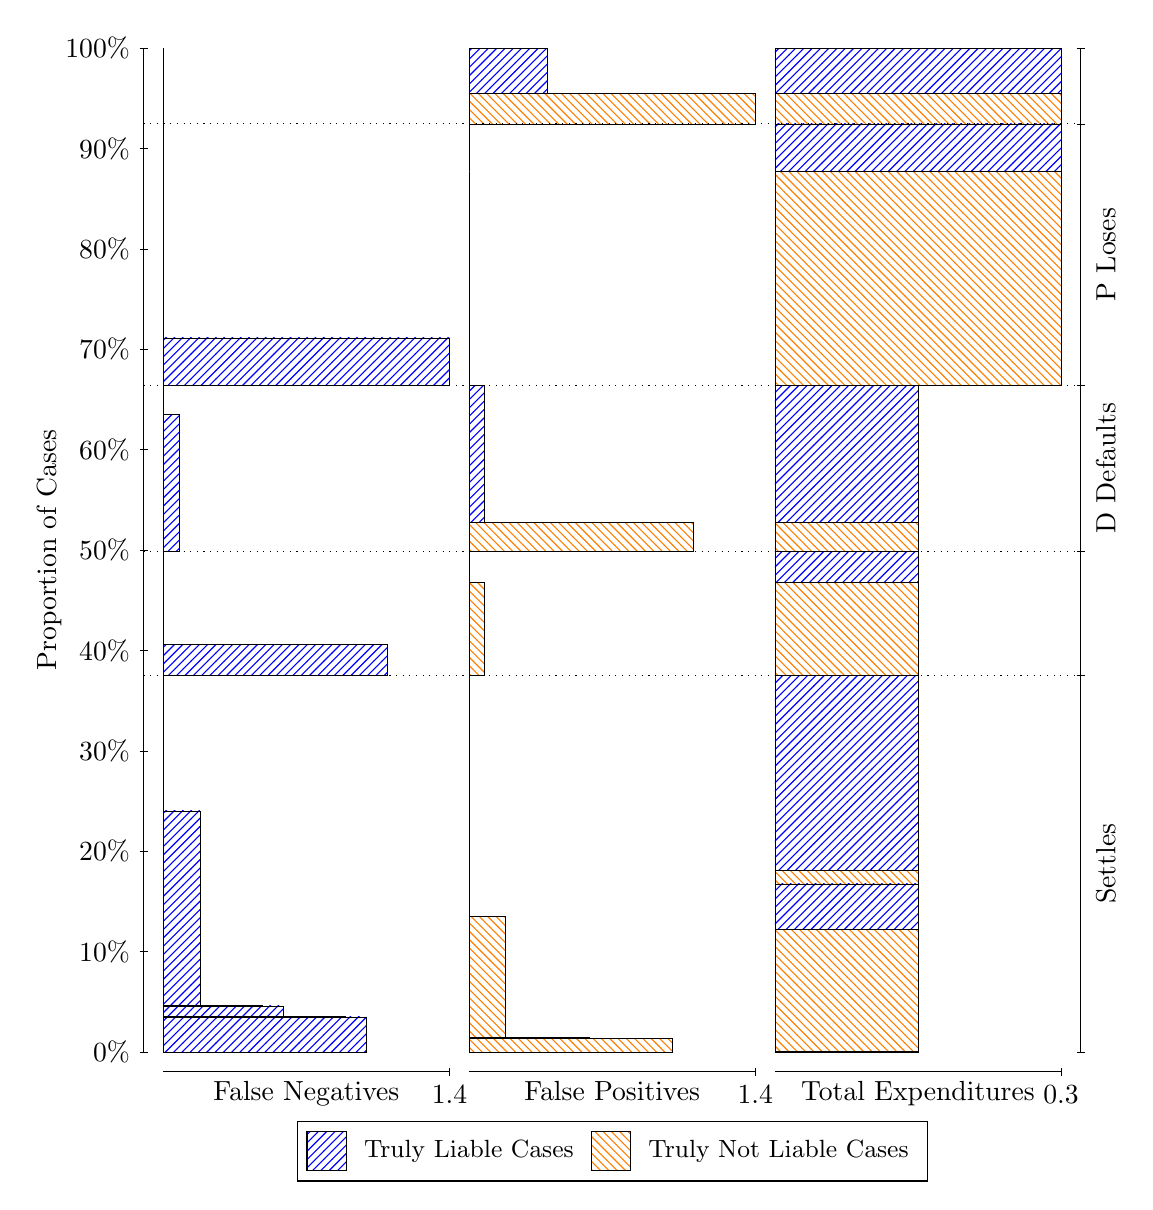
\begin{tikzpicture}
\draw[black, very thin] (1.5,1.75) -- (1.5,14.5);
\node[rotate=90, anchor=center] at (0.3, 8.125) {Proportion of Cases};
\draw[black, very thin] (1.45,1.75) -- (1.55,1.75);
\node[anchor=east] at (1.45, 1.75) {0\%};
\draw[black, very thin] (1.45,3.025) -- (1.55,3.025);
\node[anchor=east] at (1.45, 3.025) {10\%};
\draw[black, very thin] (1.45,4.3) -- (1.55,4.3);
\node[anchor=east] at (1.45, 4.3) {20\%};
\draw[black, very thin] (1.45,5.575) -- (1.55,5.575);
\node[anchor=east] at (1.45, 5.575) {30\%};
\draw[black, very thin] (1.45,6.85) -- (1.55,6.85);
\node[anchor=east] at (1.45, 6.85) {40\%};
\draw[black, very thin] (1.45,8.125) -- (1.55,8.125);
\node[anchor=east] at (1.45, 8.125) {50\%};
\draw[black, very thin] (1.45,9.4) -- (1.55,9.4);
\node[anchor=east] at (1.45, 9.4) {60\%};
\draw[black, very thin] (1.45,10.675) -- (1.55,10.675);
\node[anchor=east] at (1.45, 10.675) {70\%};
\draw[black, very thin] (1.45,11.95) -- (1.55,11.95);
\node[anchor=east] at (1.45, 11.95) {80\%};
\draw[black, very thin] (1.45,13.225) -- (1.55,13.225);
\node[anchor=east] at (1.45, 13.225) {90\%};
\draw[black, very thin] (1.45,14.5) -- (1.55,14.5);
\node[anchor=east] at (1.45, 14.5) {100\%};

\draw[black, very thin] (13.4,1.75) -- (13.4,14.5);
\draw[black, very thin] (13.35,1.75) -- (13.45,1.75);
\node[anchor=west] at (13.35, 1.75) {};
\draw[black, very thin] (13.35,6.533) -- (13.45,6.533);
\node[anchor=west] at (13.35, 6.533) {};
\draw[black, very thin] (13.35,8.1059) -- (13.45,8.1059);
\node[anchor=west] at (13.35, 8.1059) {};
\draw[black, very thin] (13.35,10.218) -- (13.45,10.218);
\node[anchor=west] at (13.35, 10.218) {};
\draw[black, very thin] (13.35,13.536) -- (13.45,13.536);
\node[anchor=west] at (13.35, 13.536) {};
\draw[black, very thin] (13.35,14.5) -- (13.45,14.5);
\node[anchor=west] at (13.35, 14.5) {};

\draw[black, very thin, pattern color=blue, pattern=north east lines] (1.75,1.75) rectangle (4.3264,2.197);
\draw[black, very thin, pattern color=blue, pattern=north east lines] (1.75,2.197) rectangle (4.0621,2.1982);
\draw[black, very thin, pattern color=blue, pattern=north east lines] (1.75,2.1982) rectangle (3.7979,2.1993);
\draw[black, very thin, pattern color=blue, pattern=north east lines] (1.75,2.1993) rectangle (3.5336,2.2005);
\draw[black, very thin, pattern color=blue, pattern=north east lines] (1.75,2.2005) rectangle (3.2694,2.3363);
\draw[black, very thin, pattern color=blue, pattern=north east lines] (1.75,2.3363) rectangle (3.0052,2.3378);
\draw[black, very thin, pattern color=blue, pattern=north east lines] (1.75,2.3378) rectangle (2.7409,2.3392);
\draw[black, very thin, pattern color=blue, pattern=north east lines] (1.75,2.3392) rectangle (2.4767,2.3407);
\draw[black, very thin, pattern color=blue, pattern=north east lines] (1.75,2.3407) rectangle (2.2124,4.812);
\draw[black, very thin, pattern color=orange, pattern=north west lines] (1.75,4.812) rectangle (1.75,6.533);
\draw[black, very thin, pattern color=blue, pattern=north east lines] (1.75,6.533) rectangle (4.5906,6.9292);
\draw[black, very thin, pattern color=orange, pattern=north west lines] (1.75,6.9292) rectangle (1.75,8.1059);
\draw[black, very thin, pattern color=blue, pattern=north east lines] (1.75,8.1059) rectangle (1.9482,9.8471);
\draw[black, very thin, pattern color=orange, pattern=north west lines] (1.75,9.8471) rectangle (1.75,10.218);
\draw[black, very thin, pattern color=blue, pattern=north east lines] (1.75,10.218) rectangle (5.3833,10.82);
\draw[black, very thin, pattern color=orange, pattern=north west lines] (1.75,10.82) rectangle (1.75,13.536);
\draw[black, very thin, pattern color=orange, pattern=north west lines] (1.75,13.536) rectangle (1.75,13.926);
\draw[black, very thin, pattern color=blue, pattern=north east lines] (1.75,13.926) rectangle (1.75,14.5);
\draw[black, very thin, pattern color=orange, pattern=north west lines] (5.6333,1.75) rectangle (8.2097,1.921);
\draw[black, very thin, pattern color=orange, pattern=north west lines] (5.6333,1.921) rectangle (7.9455,1.9211);
\draw[black, very thin, pattern color=orange, pattern=north west lines] (5.6333,1.9211) rectangle (7.6812,1.9213);
\draw[black, very thin, pattern color=orange, pattern=north west lines] (5.6333,1.9213) rectangle (7.417,1.9214);
\draw[black, very thin, pattern color=orange, pattern=north west lines] (5.6333,1.9214) rectangle (7.1527,1.9343);
\draw[black, very thin, pattern color=orange, pattern=north west lines] (5.6333,1.9343) rectangle (6.8885,1.9343);
\draw[black, very thin, pattern color=orange, pattern=north west lines] (5.6333,1.9343) rectangle (6.8885,1.9344);
\draw[black, very thin, pattern color=orange, pattern=north west lines] (5.6333,1.9344) rectangle (6.6242,1.9345);
\draw[black, very thin, pattern color=orange, pattern=north west lines] (5.6333,1.9345) rectangle (6.36,1.9346);
\draw[black, very thin, pattern color=orange, pattern=north west lines] (5.6333,1.9346) rectangle (6.0958,3.471);
\draw[black, very thin, pattern color=blue, pattern=north east lines] (5.6333,3.471) rectangle (5.6333,6.533);
\draw[black, very thin, pattern color=orange, pattern=north west lines] (5.6333,6.533) rectangle (5.8315,7.7096);
\draw[black, very thin, pattern color=blue, pattern=north east lines] (5.6333,7.7096) rectangle (5.6333,8.1059);
\draw[black, very thin, pattern color=orange, pattern=north west lines] (5.6333,8.1059) rectangle (8.4739,8.4768);
\draw[black, very thin, pattern color=blue, pattern=north east lines] (5.6333,8.4768) rectangle (5.8315,10.218);
\draw[black, very thin, pattern color=orange, pattern=north west lines] (5.6333,10.218) rectangle (5.6333,12.935);
\draw[black, very thin, pattern color=blue, pattern=north east lines] (5.6333,12.935) rectangle (5.6333,13.536);
\draw[black, very thin, pattern color=orange, pattern=north west lines] (5.6333,13.536) rectangle (9.2667,13.926);
\draw[black, very thin, pattern color=blue, pattern=north east lines] (5.6333,13.926) rectangle (6.6242,14.5);
\draw[black, very thin, pattern color=orange, pattern=north west lines] (9.5167,1.75) rectangle (11.333,1.7503);
\draw[black, very thin, pattern color=blue, pattern=north east lines] (9.5167,1.7503) rectangle (11.333,1.7538);
\draw[black, very thin, pattern color=orange, pattern=north west lines] (9.5167,1.7538) rectangle (11.333,3.303);
\draw[black, very thin, pattern color=blue, pattern=north east lines] (9.5167,3.303) rectangle (11.333,3.8859);
\draw[black, very thin, pattern color=orange, pattern=north west lines] (9.5167,3.8859) rectangle (11.333,4.0573);
\draw[black, very thin, pattern color=blue, pattern=north east lines] (9.5167,4.0573) rectangle (11.333,6.533);
\draw[black, very thin, pattern color=orange, pattern=north west lines] (9.5167,6.533) rectangle (11.333,7.7096);
\draw[black, very thin, pattern color=blue, pattern=north east lines] (9.5167,7.7096) rectangle (11.333,8.1059);
\draw[black, very thin, pattern color=orange, pattern=north west lines] (9.5167,8.1059) rectangle (11.333,8.4768);
\draw[black, very thin, pattern color=blue, pattern=north east lines] (9.5167,8.4768) rectangle (11.333,10.218);
\draw[black, very thin, pattern color=orange, pattern=north west lines] (9.5167,10.218) rectangle (13.15,12.935);
\draw[black, very thin, pattern color=blue, pattern=north east lines] (9.5167,12.935) rectangle (13.15,13.536);
\draw[black, very thin, pattern color=orange, pattern=north west lines] (9.5167,13.536) rectangle (13.15,13.926);
\draw[black, very thin, pattern color=blue, pattern=north east lines] (9.5167,13.926) rectangle (13.15,14.5);
\draw[black, dotted] (1.5,6.533) -- (13.4,6.533);
\draw[black, dotted] (1.5,8.1059) -- (13.4,8.1059);
\draw[black, dotted] (1.5,10.218) -- (13.4,10.218);
\draw[black, dotted] (1.5,13.536) -- (13.4,13.536);
\draw[black, very thin] (1.75,1.5) -- (5.3833,1.5);
\node[anchor=north] at (3.5667, 1.5) {False Negatives};
\draw[black, very thin] (5.3833,1.45) -- (5.3833,1.55);
\node[anchor=north] at (5.3833, 1.45) {1.4};

\draw[black, very thin] (5.6333,1.5) -- (9.2667,1.5);
\node[anchor=north] at (7.45, 1.5) {False Positives};
\draw[black, very thin] (9.2667,1.45) -- (9.2667,1.55);
\node[anchor=north] at (9.2667, 1.45) {1.4};

\draw[black, very thin] (9.5167,1.5) -- (13.15,1.5);
\node[anchor=north] at (11.333, 1.5) {Total Expenditures};
\draw[black, very thin] (13.15,1.45) -- (13.15,1.55);
\node[anchor=north] at (13.15, 1.45) {0.3};

\node[black, centered, rotate=90] at (13.72, 4.1415) {Settles};

\node[black, centered, rotate=90] at (13.72, 9.1619) {D Defaults};
\node[black, centered, rotate=90] at (13.72, 11.877) {P Loses};


\draw (7.449999999999999,1.5) node[draw=none] (baseCoordinate) {};
\begin{scope}[align=center]
        \matrix[scale=0.5, draw=black, below=0.5cm of baseCoordinate, nodes={draw}, column sep=0.1cm]{
            \node[rectangle, draw, minimum width=0.5cm, minimum height=0.5cm, pattern=north east lines, pattern color=blue] {}; &
            \node[draw=none, font=\small] (B) {Truly Liable Cases}; &
            \node[rectangle, draw, minimum width=0.5cm, minimum height=0.5cm, pattern=north west lines, pattern color=orange] {}; &
            \node[draw=none, font=\small] (B) {Truly Not Liable Cases}; \\
            };
\end{scope}

\end{tikzpicture}
\end{document}